\chapter{Ein anderes Kapitel}
    Hier ein anderes Kapitel
    Viele Zitate: \cite{patterson} \cite{krizhevsky} \cite{matlab} \cite{pitts} \cite{lawrence} \cite{miesbach}
    \section{Section}
        Eine Section
        \subsection{Subsection}
            \begin{figure}[h]
                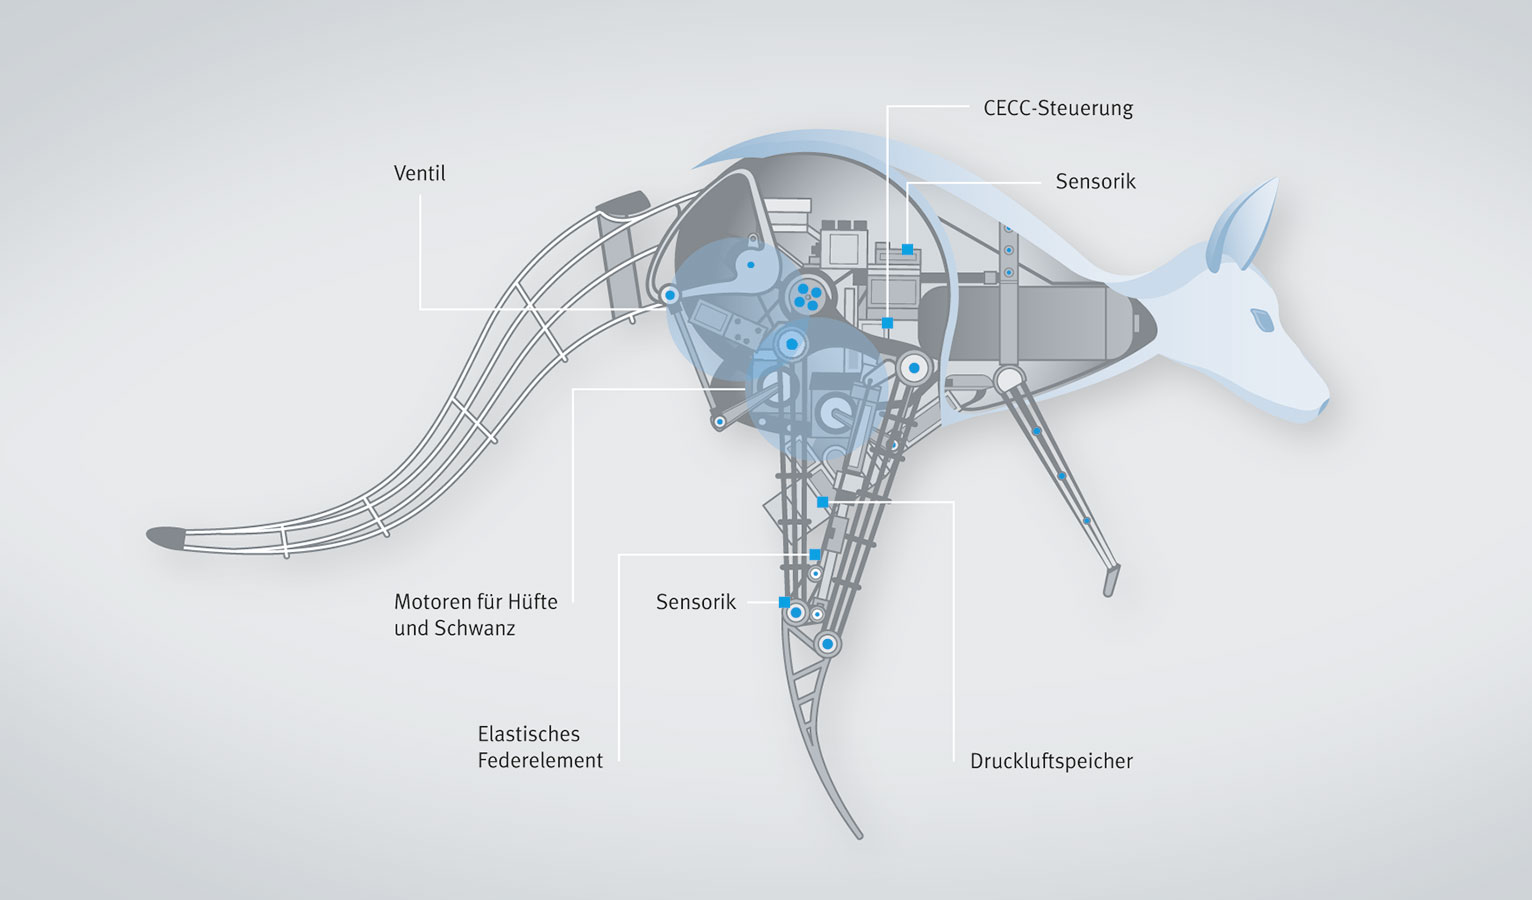
\includegraphics[scale=0.2]{Abbildungen/Kapitel2/Kangoroo.png}
                \centering
                \caption{Ein Kangoroo}
                \label{Abb:Kangoroo}   
            \end{figure}  
             \begin{table}[h]
                \begin{tabular}{ccc}
                      \hline
                      Spalte1 & Spalte2 & Spalte3\\                      
                      \hline
                      1 & 2 & 3\\
                      \hline
                \end{tabular}
                \centering
                \caption{Eine Tabelle}
                \label{Tab:Tabelle1}
            \end{table}
 
        
        
    \section{Section2}
        Eine Subsection
        \newpage
        Eine neue Seite
        \newpage 
        Noch eine neue Seite
        \newpage    
        und noch eine neue Seite